\documentclass[leqno]{beamer}
\usepackage[spanish,activeacute]{babel}
\usepackage[utf8]{inputenc}
\usepackage{amsfonts}
\usepackage{enumerate}
\usepackage{amsthm}
\usepackage{graphicx}
\usepackage{float}
\usepackage{wrapfig}
\usepackage{subfig}

\usetheme{CambridgeUS}
\usecolortheme{seahorse}

%\setbeameroption{show notes} %un-comment to see the notes

\AtBeginSection[]{
  \begin{frame}
  \vfill
  \centering
  \begin{beamercolorbox}[sep=8pt,center,shadow=true,rounded=true]{title}
    \usebeamerfont{title}\insertsectionhead\par%
  \end{beamercolorbox}
  \vfill
  \end{frame}
}

\title{Trabajo de Fin de Grado}
\subtitle{Aplicaciones prácticas del análisis de componentes principales dinámicas generalizado (Generalized Dynamic Principal Components}
\author{Anabel Gómez Ríos}

\begin{document}

\begin{frame}
\titlepage
\end{frame}

\begin{frame}
\tableofcontents
\end{frame}

\section{Objetivos}
\begin{frame}
\begin{enumerate}
	\item Comprender los principios básicos del método \textit{Generalized Dynamic Principal Components (GDPC)} y los métodos de los que deriva:
	\begin{enumerate}
		\item Análisis de componentes principales.
		\item Series temporales.
	\end{enumerate}
	\item Encontrar y llevar a cabo aplicaciones del GDPC:
	\begin{enumerate}
		\item Compresión de imágenes.
		\item Detección de patrones en series periódicas.
		\item Predicción de nuevos valores de un conjunto de series temporales.
	\end{enumerate}
\end{enumerate}
\end{frame}

\note{El análisis de componentes principales dinámicas generalizado es un método para reducir la dimensión de un conjunto de series temporales que normalmente tienen algo en común. Para poder cumplir este objetivo ha sido necesario entender el análisis de componentes principales, que es uno de los métodos más conocidos de reducción de dimensión, por ser en el que se basa el GDPC. Además, se ha necesitado tener una base de conocimientos sobre series temporales: qué son y cómo se pueden llegar a modelar.\\
En cuanto a las aplicaciones, se han llevado a cabo la compresión de imágenes, la detección de patrones en series periódicas y la predicción de nuevos valores. Con la aplicación a compresión de imágenes no se pretendía mejorar ninguno de los algoritmos ya presentes, sino utilizarlo para terminar de comprender el método, ya que se pueden hacer muchas pruebas fáciles de ver al estar tratando con imágenes.}
\note{Aun así, se han conseguido mejores resultados comprimiendo imágenes que los que se esperaban inicialmente. La segunda aplicación permite detectar patrones en series periódicas con un mínimo preprocesamiento de la serie original, lo que aventaja a otros métodos de detección de patrones. La tercera aplicación es la más interesante en tanto a que se pueden predecir nuevos valores, que es una de las prácticas más comunes del análisis de series temporales, de un conjunto de series temporales tan grande como se quiera prediciendo valores de un conjunto muy reducido: las componentes principales dinámicas. Este primer objetivo global corresponde a la parte matemática del trabajo y el segundo, a la informática.}

\section{Contenido matemático}

\begin{frame}{Análisis de componentes principales}
Sea $X = (X_1, X_2, \dots, X_n)^T$ un vector de variables aleatorias que suponemos con media cero con matriz de covarianzas $\Sigma$ semidefinida positiva y con $\lambda_1 \leq \dots \leq \lambda_p \leq 0$ las raíces características de $\Sigma$.\\

Las componentes principales son combinaciones lineales de $(X_1, \dots, X_p)$: si $l_i^T=(l_{i1}, l_{i2}, \dots, l_{ip})$, $i=1,\dots,p$ son vectores, las componentes principales son
\begin{equation*}
  \left\lbrace
  \begin{array}{l}
     Y_1 = l_1^TX = l_{11}X_1 + \cdots + l_{1p}X_p \\
     \vdots \\
     Y_p = l_p^TX = l_{p1}X_1 + \cdots + l_{pp}X_p \\
  \end{array}
  \right.
\end{equation*}
\end{frame}

\note{El análisis de componentes principales es entonces un método para reducir la dimensión de un conjunto de datos. Si se tienen $m$ datos de dimensión $n$, el análisis de componentes principales busca unos nuevos ejes, las componentes principales, que son una rotación de los antiguos, de forma que los datos representados en estos nuevos $p$ ejes tendrán sólo $p$ dimensiones. Los datos se suponen con media cero por simplicidad, ya que no es algo difícil de conseguir. Las componentes principales se buscan como combinaciones lineales de los datos originales, de forma que maximicen su varianza.}

\begin{frame}{Análisis de componentes principales}
Se impone que el módulo de los vectores $l_i,\ i=1,\dots,p$ sea uno, que las combinaciones lineales $Y_i$ sean incorreladas entre sí y que cada $Y_i$ maximice su varianza, problemas que se resolverán con multiplicadores de Lagrange.\\
Se demuestra que $Y_1 = e_1^TX$, con $e_1^Te_1=1$, $e_1$ el vector propio asociado al mayor valor propio $\lambda_1$ de $\Sigma$ y $\text{var}(Y_1) = \lambda_1$. Del mismo modo, $Y_{r+1} = e_{r+1}^T X$, con $e_{r+1}$ el vector propio asociado al valor propio $\lambda_{r+1}$, $\text{var}(Y_{r+1}) = \lambda_{r+1}$ y $1 \leq r+1 \leq p$.

\end{frame}

\note{Está demostrado en la memoria que la primera componente principal es el vector propio de la matriz de covarianzas asociado al mayor valor propio, la segunda componente principal es el vector propio asociado al segundo mayor valor propio, etc. El número de componentes, $p$, que se pueden obtener se puede fijar en función de la cantidad de información que se está dispuesto a perder.\\

De esta forma, se obtienen vectores indicando la máxima varianza de los datos, que son incorrelados entre sí, es decir, ortogonales, que funcionan como un nuevo sistema de ejes. Así, se pueden obtener las coordenadas de los datos en este nuevo sistema de ejes, que tendrán $p$ componentes, con $p$ menor que el número de componentes original, reduciendo la dimensión de los datos.}

\begin{frame}{Series temporales}
Una \textbf{serie temporal} es un conjunto de observaciones de valores de una variable generadas secuencialmente en el tiempo, normalmente a intervalos regulares: $\{y(t);\ t=1,2,\dots,N\}$.\\

Cuando una serie temporal es \textbf{estacionaria}, la media y la varianza de la misma son constantes y la covarianza entre dos muestras de la variable, $y(t)$ e $y(t+k)$ sólo depende de $k$.\\

La \textbf{ecuación general para modelar una serie temporal} es
\begin{equation}
y(t) = F(y(t-1),y(t-2),\dots, y(t-k),\dots) + e(t)
\end{equation}

Hay muchos tipos de modelos de series temporales: lineales, como los modelos AR, MA, ARMA, ARIMA, SARIMA, ARX, etc., y no lineales: funciones de base radial, perceptrones multicapa, sistemas difusos, etc.
\end{frame}

\note{Es interesante construir modelos para representar la evolución de una serie temporal, de forma que se puedan hacer predicciones sobre valores futuros de la misma. Estos modelos se basan en valores pasados de la serie y en la hipótesis de que las condiciones futuras serán análogas a las pasadas.\\
$e(t)$ es un componente aleatorio que recoge el resto de efectos que actúan sobre la serie, sobre el que se supone que las variables son independientes entre sí y que siguen una distribución normal de media cero y varianza constante.\\

Aunque hay muchos tipos de modelos para una serie temporal, en el trabajo sólo se desarrollan con un poco de profundidad los modelos AR o auto-regresivos, MA o de medias móviles y ARMA, por ser los modelos lineales más sencillos y los que se han utilizado en la segunda parte del trabajo. Para utilizar dichos métodos es necesario que la serie que se quiere modelar sea estacionaria.}

\begin{frame}{Análisis de componentes principales dinámicas generalizado}

El análisis de componentes principales dinámicas generalizado pretende hacer lo mismo que el análisis de componentes principales pero con un conjunto de series temporales, es decir, reducir la dimensión de un conjunto de series temporales. En este caso, se buscan unas nuevas series temporales, las componentes principales dinámicas, que llevarán asociadas cada una una matriz y un vector de coeficientes.\\

\begin{enumerate}
\item Antecedentes: el método de componentes principales de Brillinger.
\item No es necesario que sean combinaciones lineales de las series temporales originales. 
\item Las series originales no tienen por qué ser estacionarias.
\item Las componentes principales dinámicas se pueden obtener según las que menor error cuadrático tengan o se puede utilizar otro criterio.
\end{enumerate}

\end{frame}

\note{Antes del método de Peña, Brillinger ya había dado uno para reducir también la dimensión de un conjunto de series temporales. En su caso, las series tenían que ser estacionarias, eran combinaciones lineales de las series originales y se obtienen a través de transformadas inversas de Fourier.\\

El método de Peña es interesante porque no requiere preprocesar las series para hacerlas estacionarias y se pueden calcular las componentes principales dinámicas con cualquier criterio. Además, las componentes principales dinámicas resultantes no tienen por qué ser combinaciones lineales de las originales.}

\begin{frame}{Análisis de componentes principales dinámicas generalizado}
Sea $z_{j,t}$, $1 \leq j \leq m$, $1 \leq t \leq T$ una matriz con las series observadas, concretamente $m$ series de $T$ valores cada una.
Si $\mathbf{f} = (f_1, \dots, f_{T+k})$ es la primera componente principal dinámica, $\beta = (\beta_{j,i})_{1 \leq j \leq m, 1 \leq k+1}$ una matriz de coeficientes y $\alpha = (\alpha_1, \dots, \alpha_m)$ un vector de coeficientes, la reconstrucción de las series con dicha componente, con $k$ leads, está dada por:
\begin{equation}
\widehat{z}_{j,t} = \sum_{i=0}^{k} \beta_{j,i+1}f_{t+i} + \alpha_j
\end{equation}
\end{frame}

\note{Se utilizan $k$ valores anteriores o posteriores de cada serie para reconstruir cada valor de las series originales. Está demostrado en la memoria que es equivalente usar $k$ lags (valores anteriores) como $k$ leads (valores posteriores). Si la reconstrucción se quiere hacer con más de una componente, se suman las reconstrucciones que se hacen con cada una de ellas.\\

En la memoria se da el algoritmo iterativo que dan Peña y Yohai, autores del artículo, para extraer tanto las componentes principales como los coeficientes de cada componente.\\

El número de componentes principales se puede elegir, como en el análisis de componentes principales, en función de la cantidad de información que se está dispuesto a perder.}

\section{Contenido informático}

\begin{frame}{Descripción de las herramientas utilizadas}
Se han utilizado principalmente:
\begin{enumerate}
\item \texttt{R}
\item Paquete \texttt{gdpc} en desarrollo disponible en el git de Ezequiel Smucler.
\item Funciones en \texttt{R} hechas por mí para la reconstrucción de series, automatización de pruebas, etc.
\end{enumerate}
\end{frame}

\note{Se ha utilizado principalmente \texttt{R}, excepto para hacer los test ANOVA y rangos múltiples, que se ha utilizado una versión de prueba de Statgraphics, por simplicidad. Todo lo que hay sobre el paquete \texttt{gdpc} está en desarrollo. Empecé utilizando una versión que me facilitó Daniel Peña, pero tenía fallos y me puse en contacto con el que mantiene el paquete, Ezequiel Smucler, y me refirió a la versión que tenía él en su git, que aunque sigue en desarrollo y de hecho ya hay cambios con respecto a lo que yo he utilizado, funcionaba bastante mejor. Este paquete obtiene las componentes principales dinámicas y las matrices y vectores de coeficientes que se han comentado antes. La reconstrucción de las series, la automatización de pruebas para comprobar tiempos de ejecución y el resto de aplicaciones que vamos a ver aquí están programadas en \texttt{R} por mí.}

\note{En el paquete \texttt{gdpc} se pueden obtener las componentes principales dinámicas según se quiera explicar un mínimo de varianza en las series originales, el número de cores que se quieren utilizar para las partes que están paralelizadas en el código, o si se quieren obtener las \texttt{x} primeras componentes exactamente. Además, permite dar un k máximo de forma que prueba con todos los k entre 1 y el máximo dado y se queda con el que menor error tenga según el criterio escogido. Todas las pruebas que he hecho han sido con el criterio de mínimos cuadrados, por ser el que se explicaba en el paper de peña y el que mejores resultados daba.}

\begin{frame}{Análisis de tiempos del algoritmo GDPC}
\begin{table}[]
\centering
\caption{Extracto de tiempos por tipo}
\label{tiemposPorTipo}
\resizebox{\textwidth}{!}{\begin{tabular}{cccc|cccc|cccc}
Tipo       & T   & m  & Tiempo & Tipo       & T   & m   & Tiempo & Tipo       & T   & m   & Tiempo \\ \hline
MonteCarlo & 32  & 32 & 0.8    & MonteCarlo & 512 & 32  & 16.91  & MonteCarlo & 256 & 256 & 10     \\ \hline
Aleatorio  & 32  & 32 & 3.16   & Aleatorio  & 512 & 32  & 442.73 & Aleatorio  & 256 & 256 & 923.92 \\ \hline
Imagen     & 32  & 32 & 1.66   & Imagen     & 512 & 32  & 52.25  & Imagen     & 256 & 256 & 216.38 \\ \hline
MonteCarlo & 256 & 32 & 3.23   & MonteCarlo & 32  & 256 & 1.81   &            &     &     &        \\ \hline
Aleatorio  & 256 & 32 & 65.72  & Aleatorio  & 32  & 256 & 24.59  &            &     &     &        \\ \hline
Imagen     & 256 & 32 & 7.41   & Imagen     & 32  & 256 & 6.88   &            &     &     &       
\end{tabular}}
\end{table}
\end{frame}

\note{Esta tabla es una parte de la tabla de tiempos por tipo, ya que entera no entraba. En la tabla completa también se varía el parámetro expl\_var, aunque aquí se han tomado las filas correspondientes al valor 0.95 de este parámetro, por ser en el que mejor se ven las diferencias en los tiempos según el tipo de series que se utilizan. Como se puede ver, y se ha comprobado con un test ANOVA, hay bastante diferencia en tiempos entre usar series aleatorias y series generadas con un método de Monte Carlo o series sacadas de una imagen. Además, también es mayor el tiempo que tarda con series sacadas de imágenes según el número de series (m) o el número de valores en cada serie (T) aumenta.}

\begin{frame}{Análisis de tiempos del algoritmo GDPC}
\begin{table}[]
\centering
\caption{Extracto de tiempos en imágenes}
\label{tiemposimg}
\resizebox{\textwidth}{!}{\begin{tabular}{|cccc|cccc|cccc|}
\hline
ncores & T   & m  & Tiempo & ncores & T   & m   & Tiempo  & ncores & T   & m   & Tiempo  \\ \hline
1      & 32  & 32 & 1.66   & 1      & 32  & 256 & 6.88    & 1      & 32  & 512 & 9.33    \\ \hline
2      & 32  & 32 & 1.68   & 2      & 32  & 256 & 5.3     & 2      & 32  & 512 & 6.46    \\ \hline
4      & 32  & 32 & 2.28   & 4      & 32  & 256 & 4.75    & 4      & 32  & 512 & 5.2     \\ \hline
1      & 256 & 32 & 7.41   & 1      & 256 & 256 & 216.38  & 1      & 256 & 512 & 582.12  \\ \hline
2      & 256 & 32 & 5.11   & 2      & 256 & 256 & 131.44  & 2      & 256 & 512 & 363.26  \\ \hline
4      & 256 & 32 & 4.97   & 4      & 256 & 256 & 88.65   & 4      & 256 & 512 & 255.39  \\ \hline
1      & 512 & 32 & 52.25  & 1      & 512 & 256 & 1402.19 & 1      & 512 & 512 & 3116.42 \\ \hline
2      & 512 & 32 & 31.23  & 2      & 512 & 256 & 917.4   & 2      & 512 & 512 & 2246.37 \\ \hline
4      & 512 & 32 & 24.09  & 4      & 512 & 256 & 865.88  & 4      & 512 & 512 & 2543.5  \\ \hline
\end{tabular}}
\end{table}
\end{frame}

\note{Esta tabla también es un extracto de la tabla que analizaba el tiempo por parámetros, ya que la original tenía 243 filas y variaba también los parámetros \texttt{expl\_var} y \texttt{k\_max}. Aquí se ha optado por coger las filas con una varianza mínima de 0.95 y un k máximo de 7, por ser lo más cercano a lo que se ha utilizado después en las aplicaciones. Se muestra la diferencia de tiempos según el número de cores porque en el análisis ANOVA para esta tabla (aunque con los tiempos para series de Monte Carlo) decía que no el número de cores no influía en el tiempo. Sin embargo yo creo que esto es así porque cuando hay pocas series con pocos valores cuesta más paralelizar que lo que se gana paralelizando, pero cuando aumentan, sí que hay una diferencia significativa con más cores: pasamos de casi 52 minutos con 512 series de 512 valores y un core a poco más de 42 minutos con 4 cores. Aquí además están puestos los tiempos para imágenes para que se vieran los tiempos que se pueden obtener cuando se utilizan imágenes.}

\begin{frame}{Aplicación a compresión de imágenes}
\begin{figure}[H]
 \centering
  \subfloat[Imagen original]{
   \label{f:lenaO}
    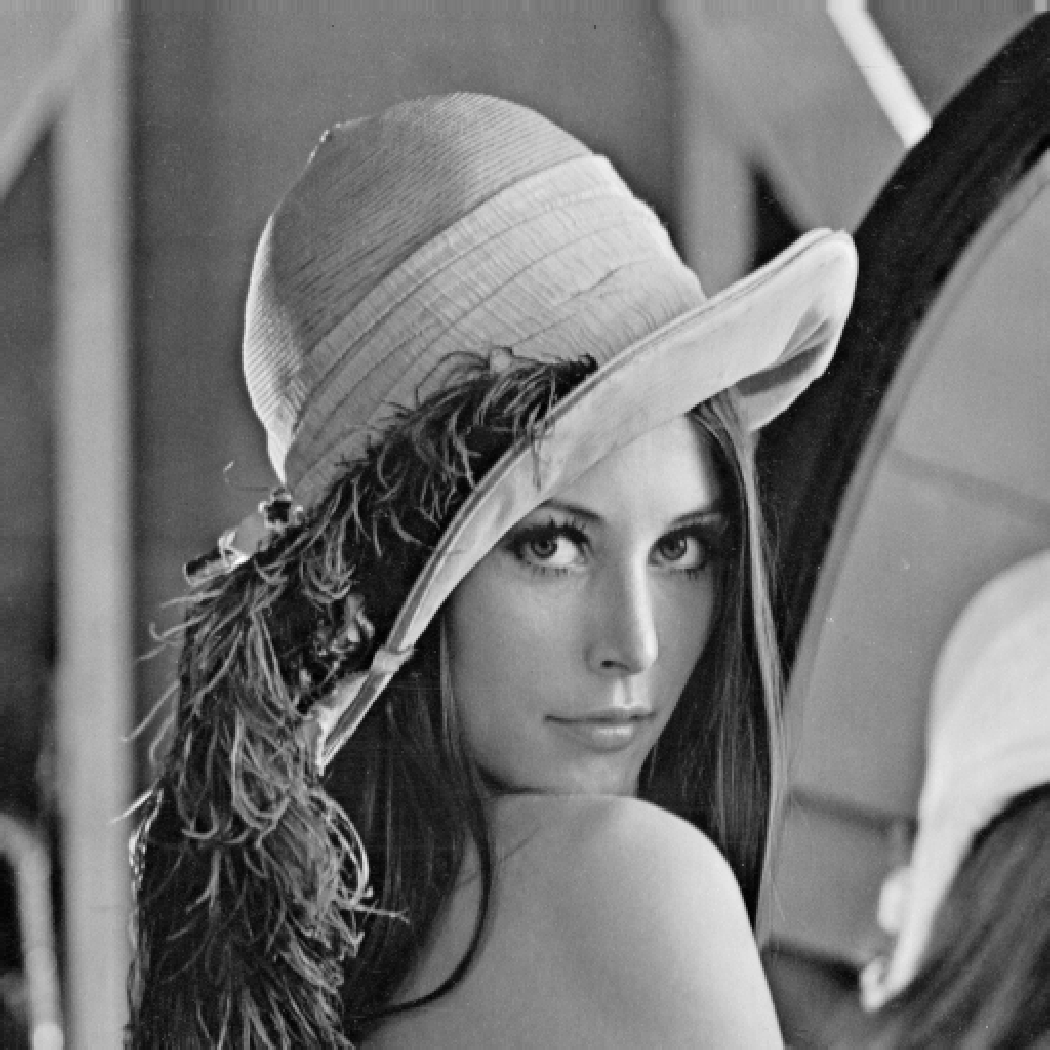
\includegraphics[width=0.45\textwidth]{../imagenes/LenaOriginal.pdf}}
  \subfloat[Imagen reconstruida]{
   \label{f:lenaR}
    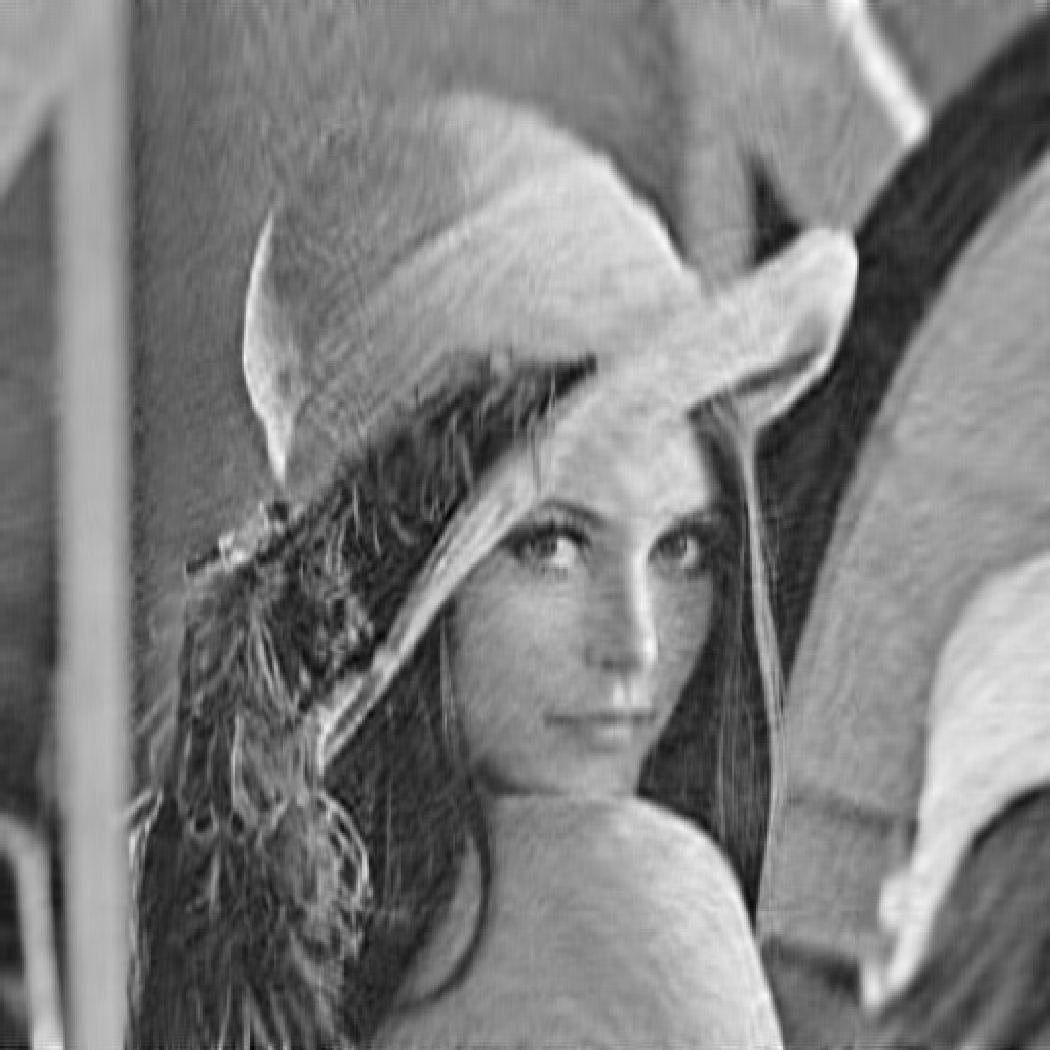
\includegraphics[width=0.45\textwidth]{../imagenes/lena095.pdf}}
 \caption{Lena}
 \label{f:imgsLena}
\end{figure}
\end{frame}

\note{Todas las imágenes se han hecho explicando un mínimo de 0.95 de varianza de las series, con un k máximo de 5 para no aumentar mucho el tiempo de ejecución y cogiendo como series las columnas de la imagen. Aquí vemos la imagen en blanco y negro que se ha utilizado. Se han hecho pruebas con esta y con dos imágenes a color. Vemos aquí la reconstrucción de la imagen habiendo cogido como series temporales las columnas de la imagen. La función para reconstruir las series temporales originales con una y con varias componentes principales está hecha por mí y se puede encontrar en mi git.}

\begin{frame}{Aplicación a compresión de imágenes}
\begin{figure}
 \centering
  \subfloat[Imagen original]{
   \label{f:patoO}
    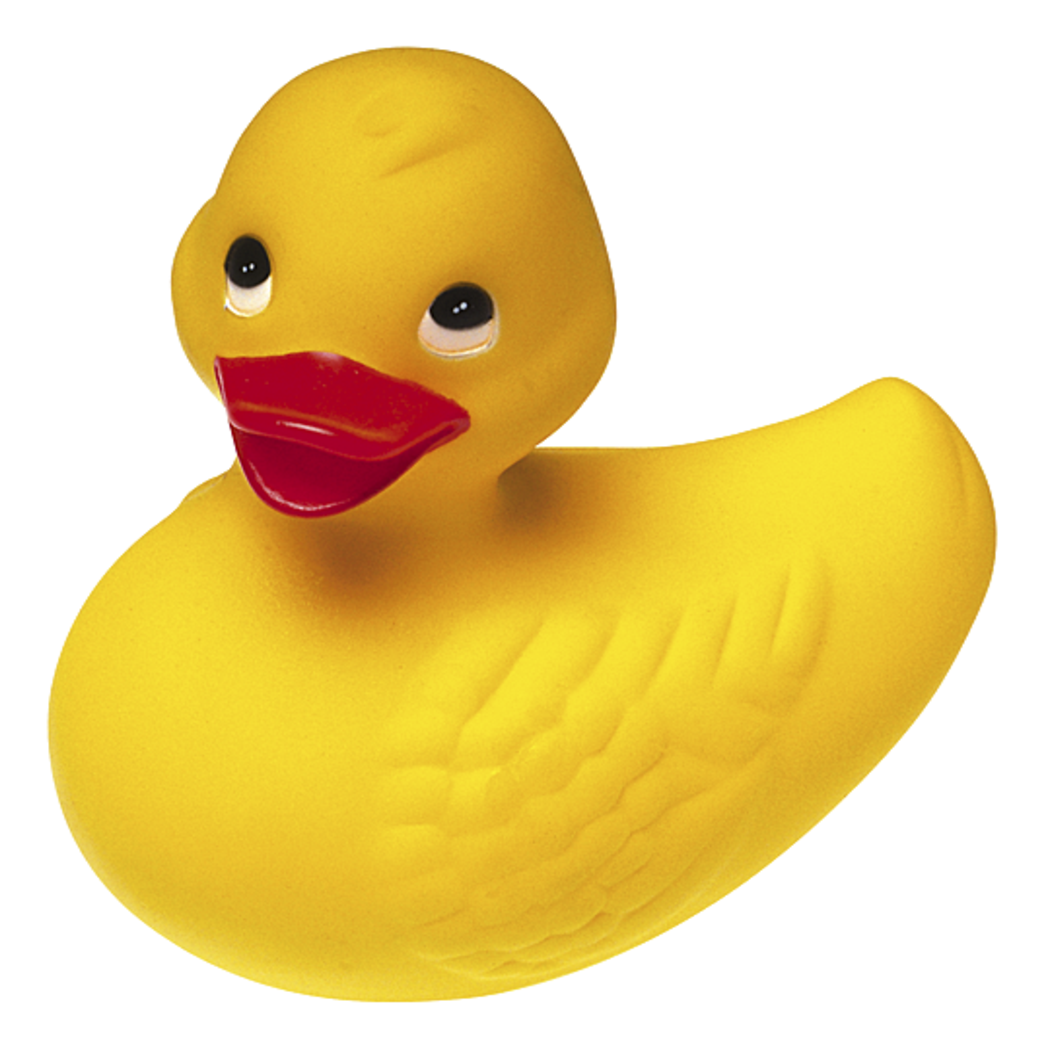
\includegraphics[width=0.45\textwidth]{../imagenes/duckOriginal.pdf}}
  \subfloat[Imagen reconstruida]{
   \label{f:patoR}
    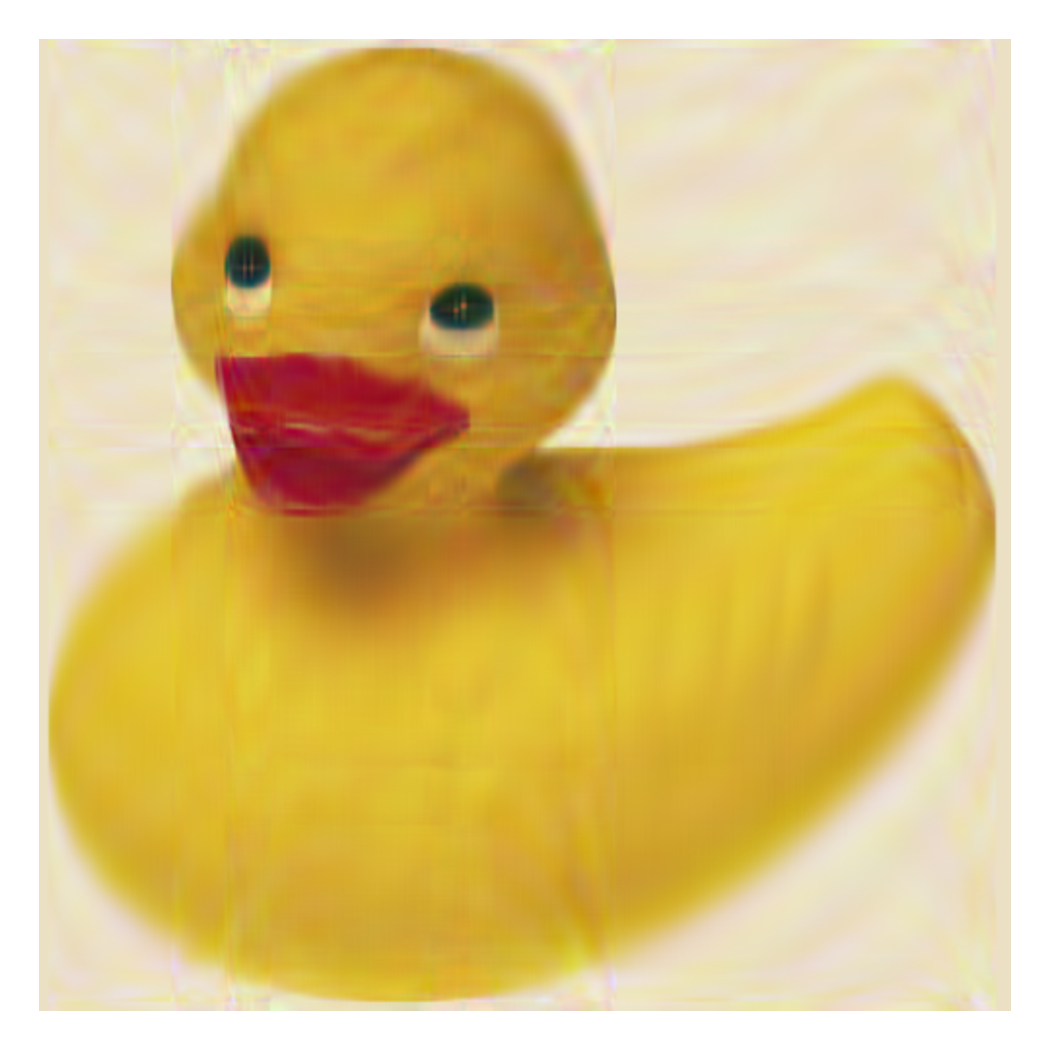
\includegraphics[width=0.45\textwidth]{../imagenes/duck095.pdf}}
 \caption{Pato}
 \label{f:imgsPato}
\end{figure}
\end{frame}

\note{Para las imágenes en color se ha hecho lo mismo pero a cada canal de color R, G y B. Como la reconstrucción de las imágenes no tiene por qué devolver valores en el rango [0,1], de hecho las imágenes originales estaban en el intervalo [0,255], se ha transformado el intervalo [min,max] de cada matriz en el intervalo [0,1] con una función de R hecha por mí.\\

En esta imagen podemos ver que no por ser la imagen más simple se obtienen mejores resultados. De hecho, si los cambios en el color o el tono de la imagen son suaves, normalmente no se ven reflejados en las series reconstruidas porque la varianza de los datos ahí es muy pequeña.}

\begin{frame}{Aplicación a compresión de imágenes}
\begin{figure}
 \centering
  \subfloat[Imagen original]{
   \label{f:tigreO}
    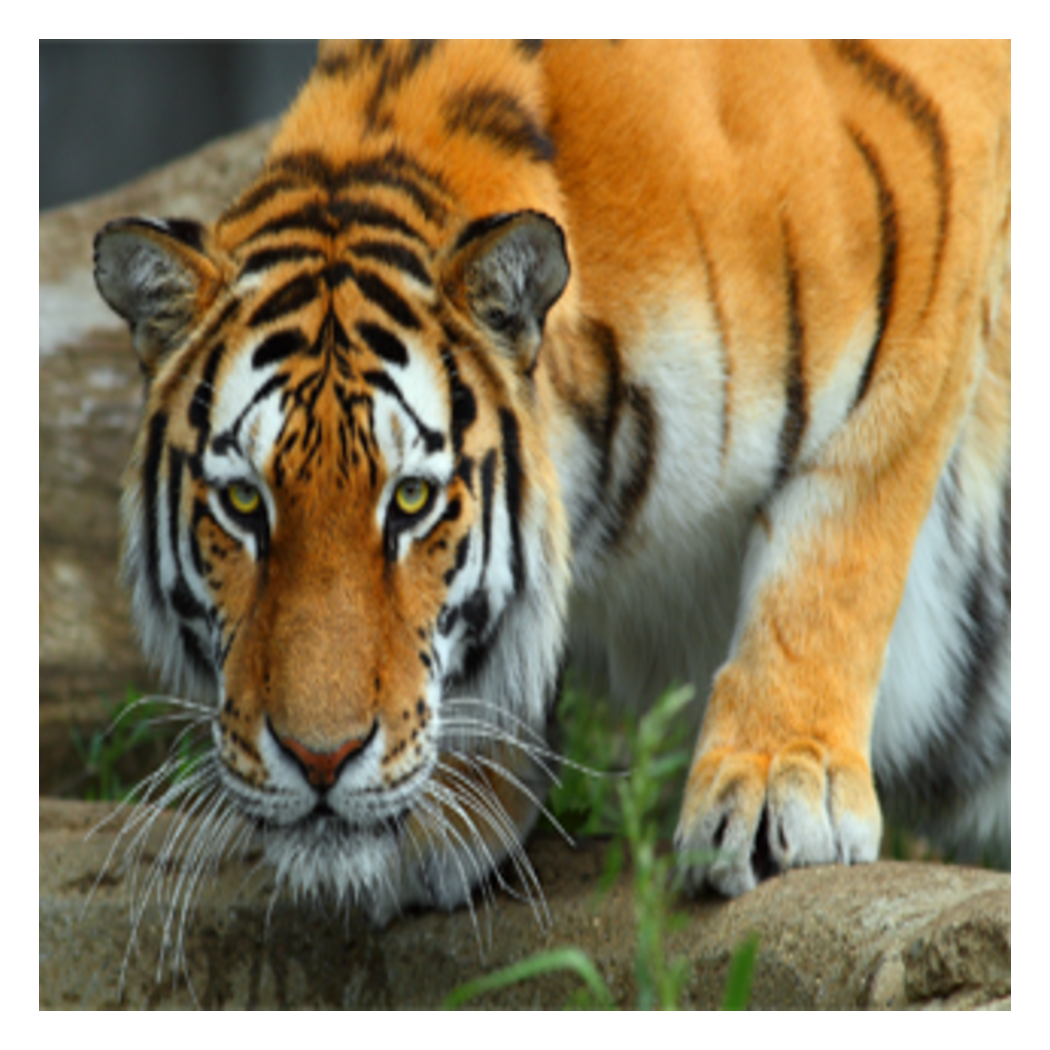
\includegraphics[width=0.45\textwidth]{../imagenes/tigerOriginal.pdf}}
  \subfloat[Imagen reconstruida]{
   \label{f:tigreR}
    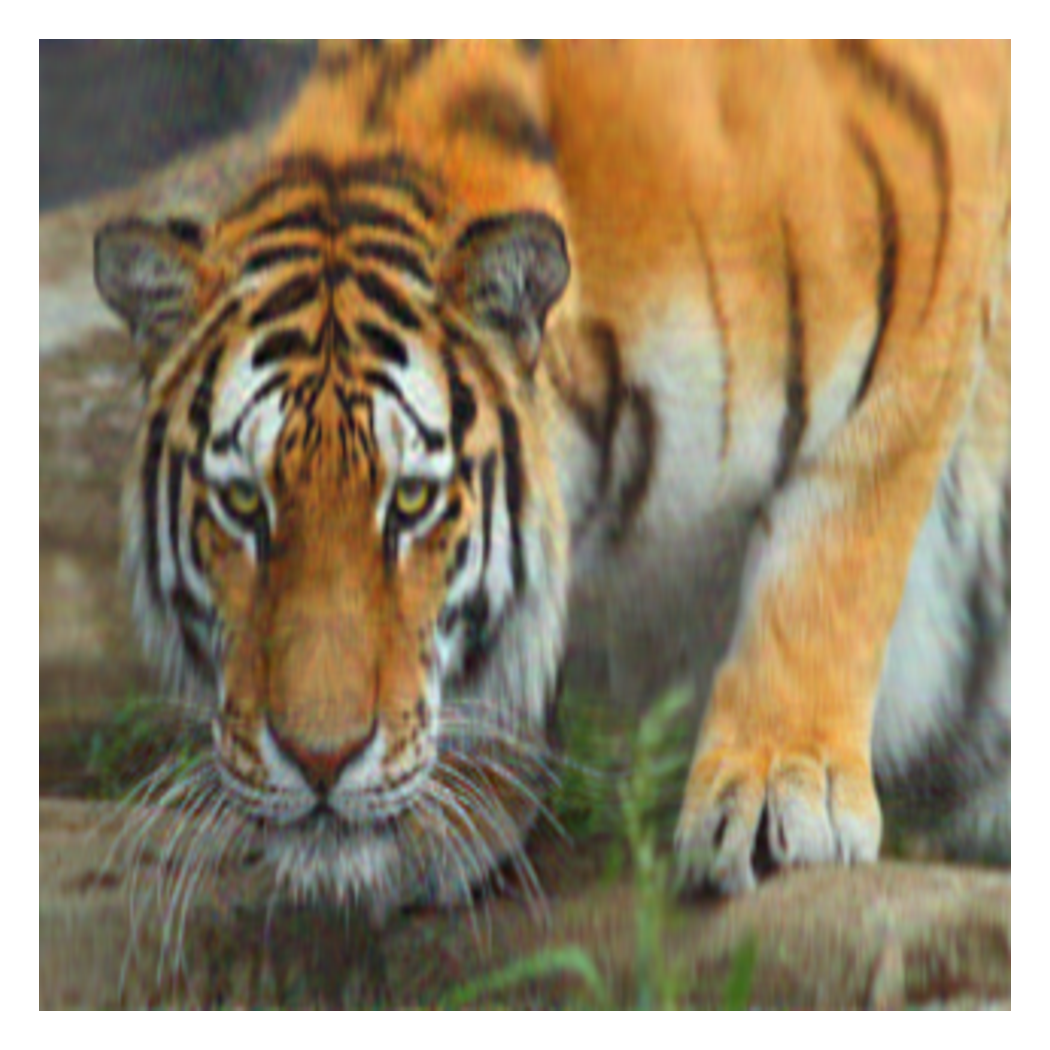
\includegraphics[width=0.45\textwidth]{../imagenes/tiger.pdf}}
 \caption{Tigre}
 \label{f:imgsTigre}
\end{figure}
\end{frame}

\note{Sin embargo, si hay cambios bruscos en los tonos, como pasa aquí, sí que aparecen en las series reconstruidas. Esto se ha comprobado modificando la imagen de Lena, como podemos ver en las siguiente imágenes.} 

\begin{frame}{Aplicación a compresión de imágenes}
\begin{figure}
 \centering
  \subfloat[Imagen original]{
   \label{f:lenaN2O}
    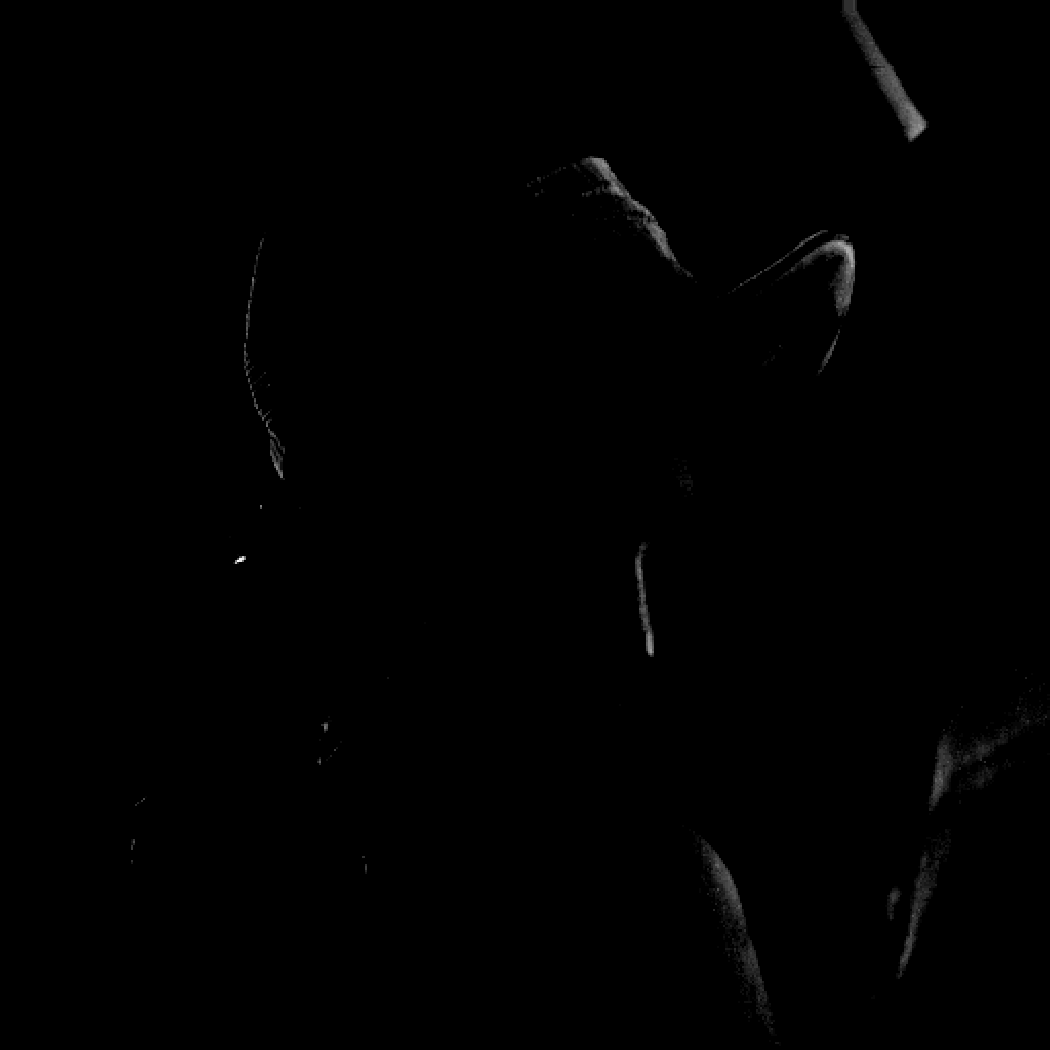
\includegraphics[width=0.45\textwidth]{../imagenes/nivelesLena2.pdf}}
  \subfloat[Imagen reconstruida]{
   \label{f:lenaN2R}
    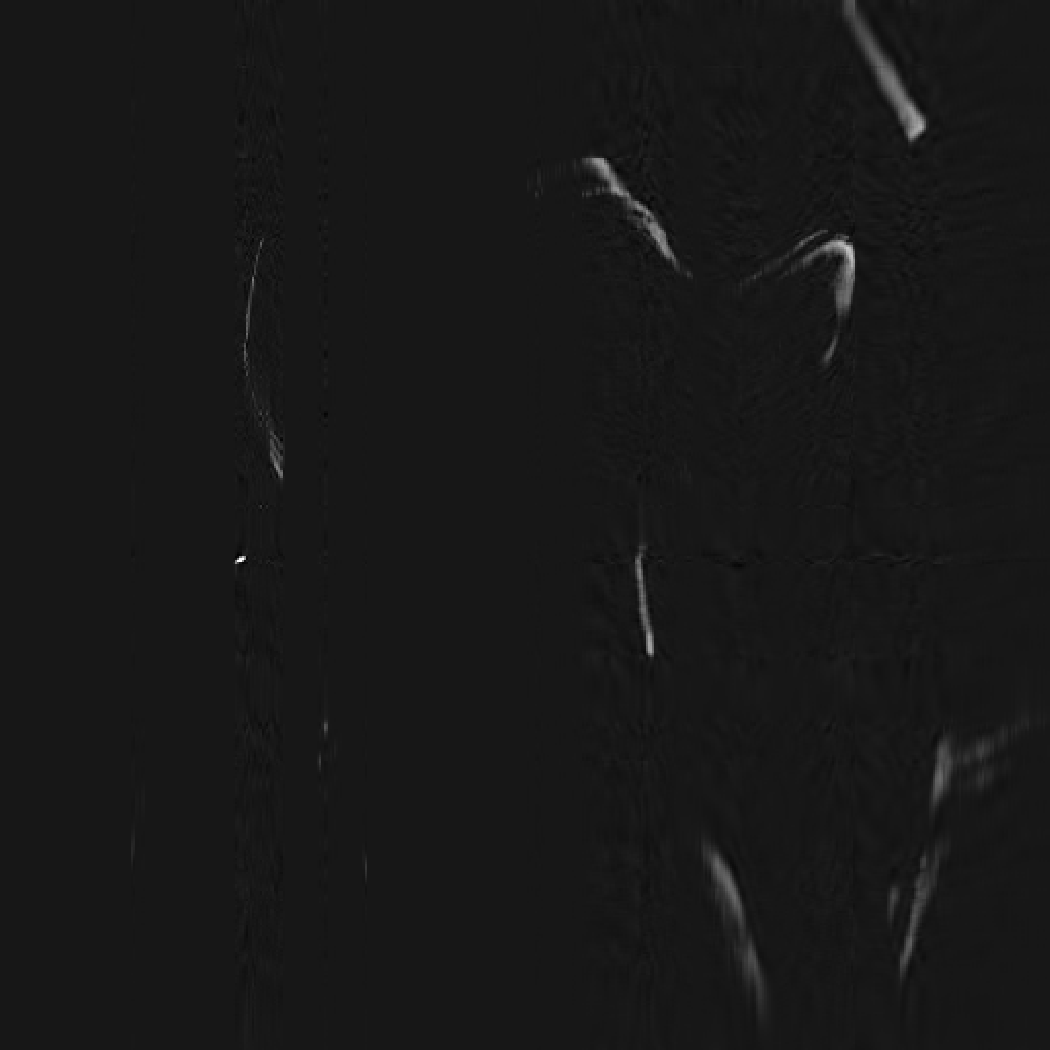
\includegraphics[width=0.45\textwidth]{../imagenes/nivelesLena2r.pdf}}
 \caption{Niveles de Lena}
 \label{f:imgsLenaN2}
\end{figure}
\end{frame}

\note{Como vemos, si los cambios son muy bruscos, se reconstruyen casi perfectamente.}

\begin{frame}{Aplicación a compresión de imágenes}
\begin{figure}
 \centering
  \subfloat[Imagen original]{
   \label{f:lenaN4O}
    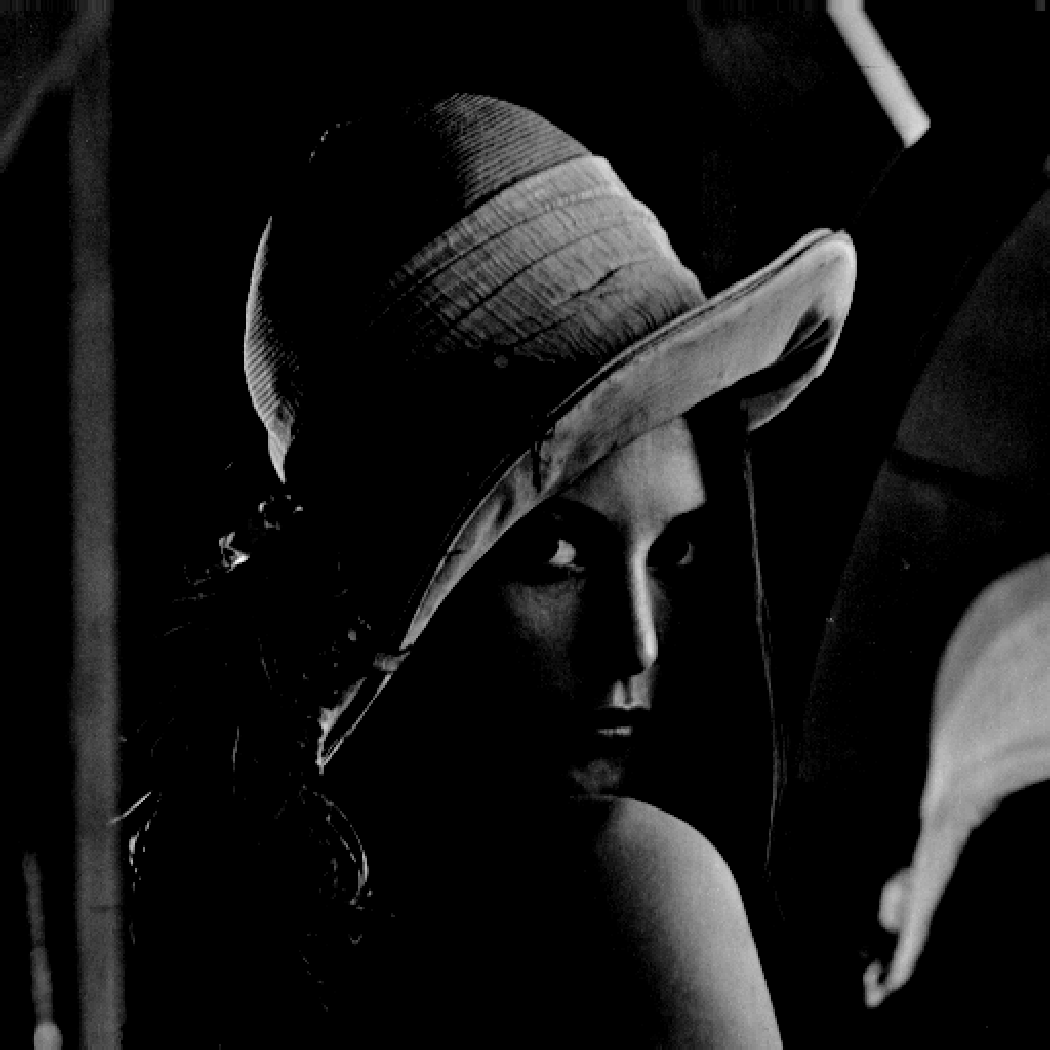
\includegraphics[width=0.5\textwidth]{../imagenes/nivelesLena4.pdf}}
  \subfloat[Imagen reconstruida]{
   \label{f:lenaN4R}
    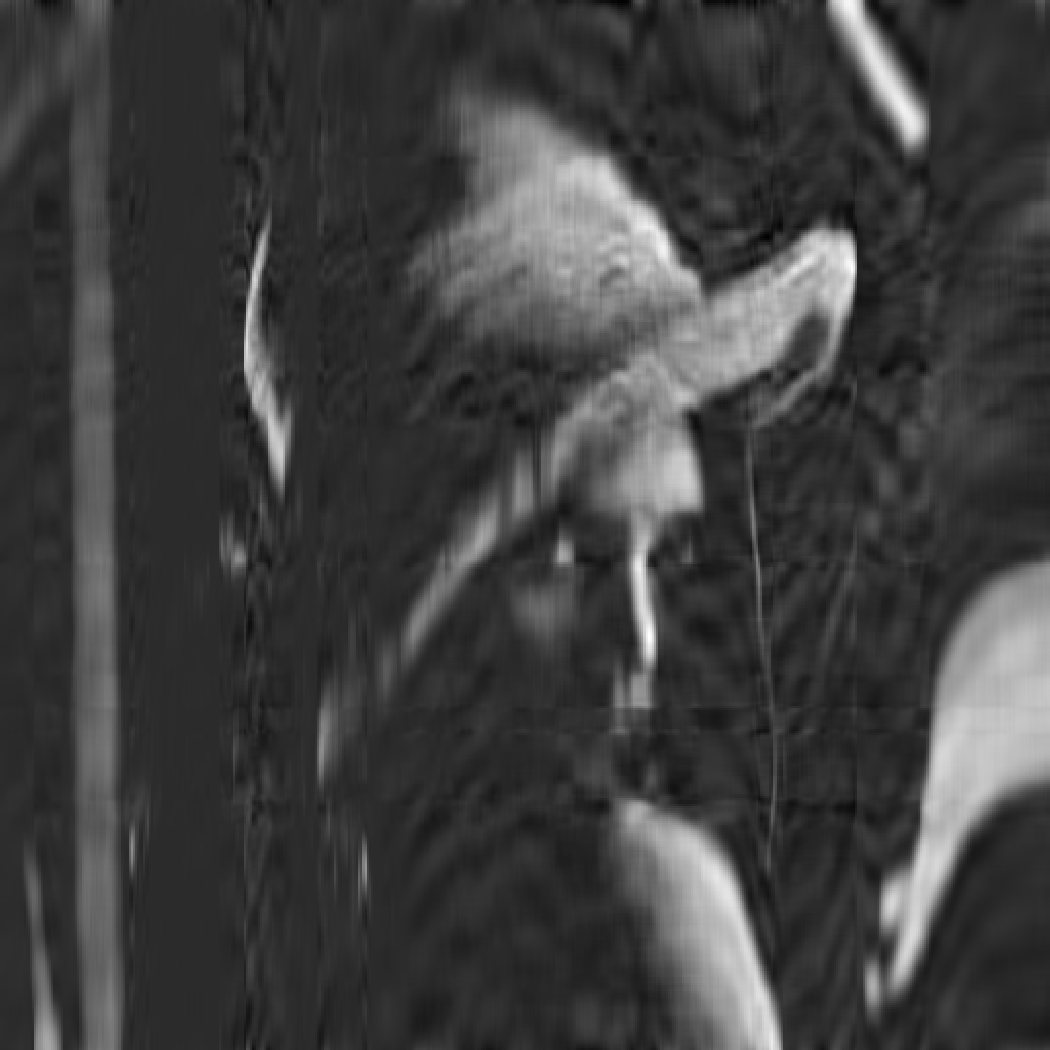
\includegraphics[width=0.5\textwidth]{../imagenes/nivelesLena4r.pdf}}
 \caption{Niveles de Lena}
 \label{f:imgsLenaN4}
\end{figure}
\end{frame}

\note{Sin embargo, según hay más grises y no suficientes detalles en la imagen, se va viendo peor. Sobre todo las partes más o menos constantes, que son las que peor se ven. Por otro lado, la imagen del tigre se veía mejor porque hacen falta más componentes principales dinámicas en esa imagen que en la del pato para explicar casi el mismo porcentaje de varianza, siendo el tigre una imagen más pequeña, como podemos ver en el siguiente cuadro}

\begin{frame}{Aplicación a compresión de imágenes}
\begin{table}[]
\centering
\caption{Factor de compresión}
\label{t:compresion}
\resizebox{\textwidth}{!}{\begin{tabular}{|cc|c|c|c|c|c|c|c|c|}
\hline
                            &         & T   & m   & \begin{tabular}[c]{@{}c@{}}nº\\ componentes\end{tabular} & \begin{tabular}[c]{@{}c@{}}k utilizados\\ (por orden)\end{tabular}                  & nº a almacenar & \begin{tabular}[c]{@{}c@{}}Total en\\ reconstruida\end{tabular} & \begin{tabular}[c]{@{}c@{}}Total en \\ original\end{tabular} & \begin{tabular}[c]{@{}c@{}}Factor de \\ compresión\end{tabular} \\ \hline
Lena                        &         & 512 & 512 & 12                                                       & \begin{tabular}[c]{@{}c@{}}5, 3, 5, 4, 5, 4, \\ 5, 4, 5, 5, 5, 5\end{tabular}       & 46647          & 46647                                                           & 262144                                                       & 5,61974                                                         \\ \hline
\multicolumn{1}{|c|}{}      & Canal R & 546 & 500 & 6                                                        & 4, 4, 5, 4, 5, 5                                                                    & 22803          &                                                                 &                                                              &                                                                 \\ \cline{2-7}
\multicolumn{1}{|c|}{Pato}  & Canal G & 546 & 500 & 5                                                        & 3, 4, 5, 5, 5                                                                       & 18752          & 62855                                                           & 819000                                                       & 13,02999                                                        \\ \cline{2-7}
\multicolumn{1}{|c|}{}      & Canal B & 546 & 500 & 6                                                        & 2, 4, 4, 4, 5, 5                                                                    & 21300          &                                                                 &                                                              &                                                                 \\ \hline
\multicolumn{1}{|c|}{}      & Canal R & 240 & 320 & 10                                                       & \begin{tabular}[c]{@{}c@{}}4, 5, 5, 5, 5, \\ 5, 5, 5, 5, 5\end{tabular}             & 24529          &                                                                 &                                                              &                                                                 \\ \cline{2-7}
\multicolumn{1}{|c|}{Tigre} & Canal G & 240 & 320 & 13                                                       & \begin{tabular}[c]{@{}c@{}}5, 5, 5, 5, 5, \\ 5, 5, 5, 5, 5, \\ 4, 5, 4\end{tabular} & 31663          & 82885                                                           & 230400                                                       & 2,779755                                                        \\ \cline{2-7}
\multicolumn{1}{|c|}{}      & Canal B & 240 & 320 & 11                                                       & \begin{tabular}[c]{@{}c@{}}4, 5, 5, 5, 5, \\ 5, 4, 5, 5, 5, 5\end{tabular}          & 26693          &                                                                 &                                                              &                                                                 \\ \hline
\end{tabular}}
\end{table}
\end{frame}

\note{Efectivamente, hacen falta casi la mitad de componentes para una imagen casi el doble de grande que la del tigre. El factor de compresión depende de lo simple que sea la imagen y de lo grande que sea también, pero aquí hemos obtenido como mínimo un factor de compresión de más de 3. Esta tabla está obtenida según los números que hace falta guardar en cada caso, teniendo en cuenta que las imágenes originales son matrices y que las comprimidas son las componentes principales dinámicas junto con sus matrices y vectores de coeficientes.}

\begin{frame}{Aplicación a compresión de imágenes}
\begin{figure}[]
 \centering
  \subfloat[Componente 1]{
   \label{f:lena0951}
    \includegraphics[width=0.33\textwidth]{../imagenes/lena0951.pdf}}
  \subfloat[Componentes 1 a 6]{
   \label{f:lena0952}
    \includegraphics[width=0.33\textwidth]{../imagenes/lena0956.pdf}}
  \subfloat[Componentes 1 a 12]{
   \label{f:lena0953}
    \includegraphics[width=0.33\textwidth]{../imagenes/lena09512.pdf}}
 \caption{Reconstrucciones de Lena con distintas componentes}
 \label{f:RLenaC1}
\end{figure}
\end{frame}

\note{Como se ha dicho anteriormente, si se tiene más de una componente principal dinámica, la reconstrucción de las series originales se lleva a cabo sumando la información que aporta para cada casilla de la matriz cada componente principal dinámica. Esto se ve muy bien con imágenes, porque es fácil visualizar los resultados. Aquí podemos ver las reconstrucciones con la primera componente sólo, con las componentes de la 1 a la 6 y con las componentes de la 1 a la 12, y podemos ver la mejora que hay según se va añadiendo la información que aporta cada componente principal dinámica.}

\begin{frame}{Aplicación a detección de patrones en series temporales periódicas}
\begin{figure}[]
 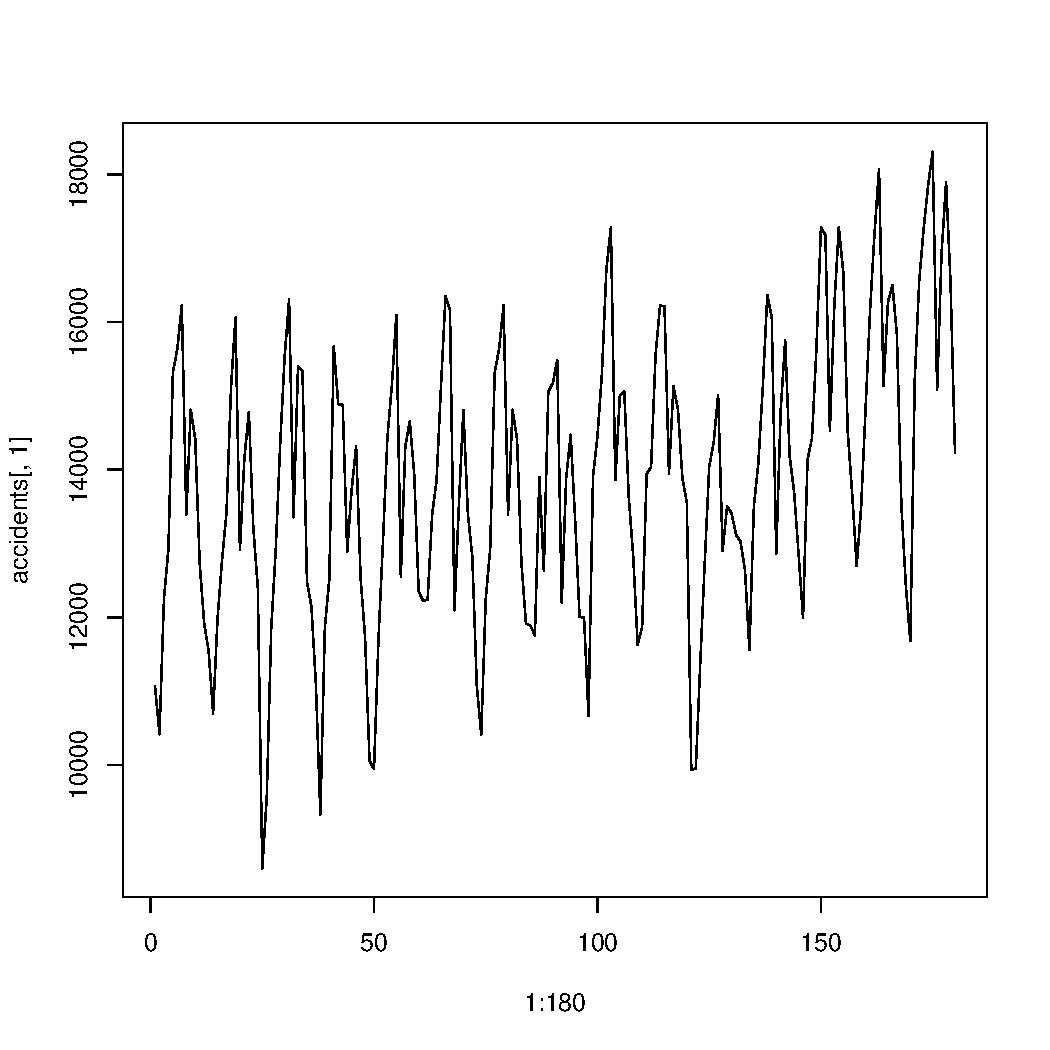
\includegraphics[width=0.9\textwidth, height=0.6\textheight]{../imagenes/accidents.pdf}
 \caption{Número mensual de accidentes de coche en Italia de 1983 a 1997}
 \label{f:accidents}
\end{figure}
\end{frame}

\note{Esta aplicación es interesante porque se pueden obtener patrones de series periódicas, que es una práctica común cuando se quiere descomponer una serie en parte periódica, tendencia, estacionaria, etc., con un preprocesamiento mínimo y automático de la serie. Lo que se hace es partir la serie original en intervalos periódicos y tratar cada intervalo como una serie independiente. Por ejemplo aquí esta serie tiene periodicidad anual, porque lo que cogeríamos cada 13 puntos de la serie original, de Enero de un año a Enero del siguiente, y tomaríamos cada 13 datos como series independientes.}

\begin{frame}{Aplicación a detección de patrones en series temporales periódicas}
\begin{figure}[]
 \centering
  \subfloat[Primer periodo]{
   \label{f:periodo1}
    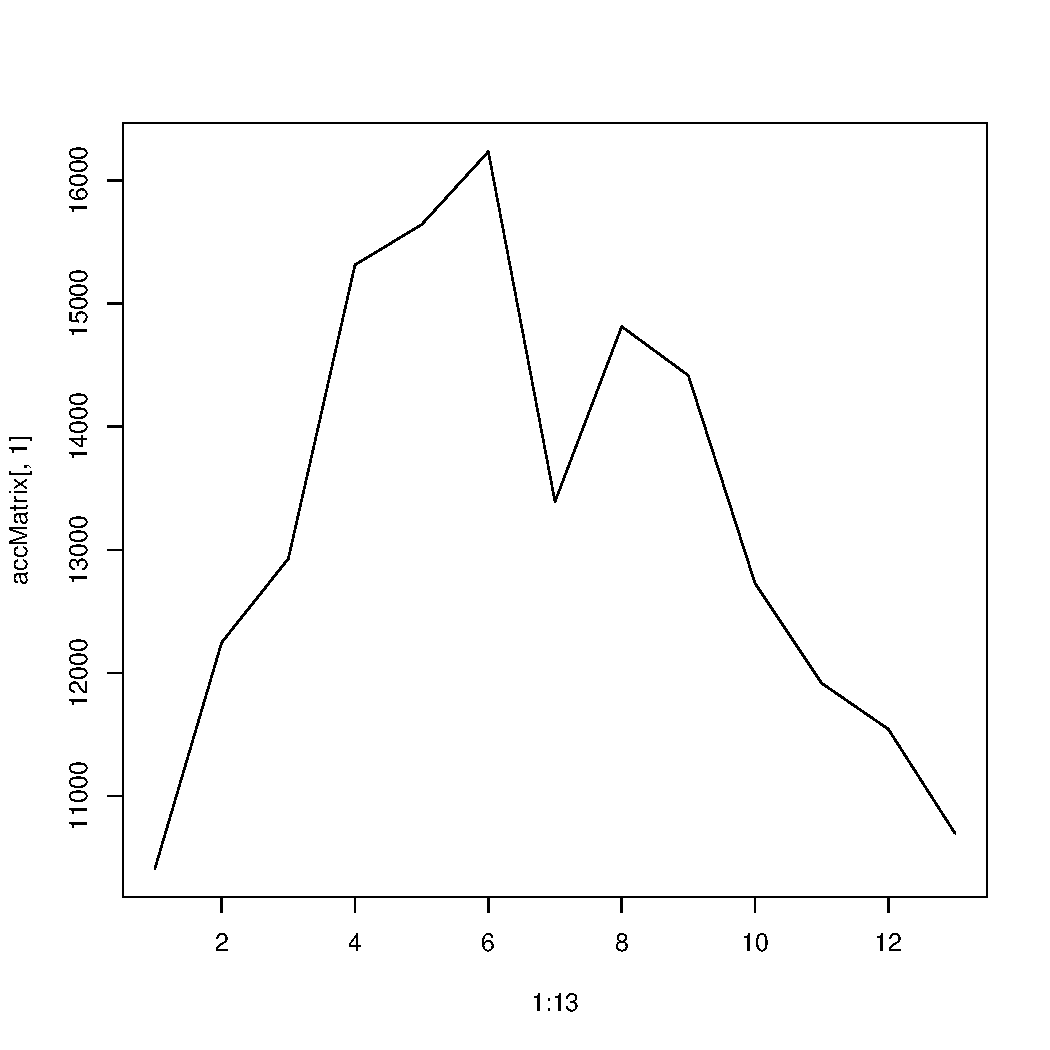
\includegraphics[width=0.33\textwidth]{../imagenes/primerPeriodo.pdf}}
  \subfloat[Segundo periodo]{
   \label{f:periodo2}
    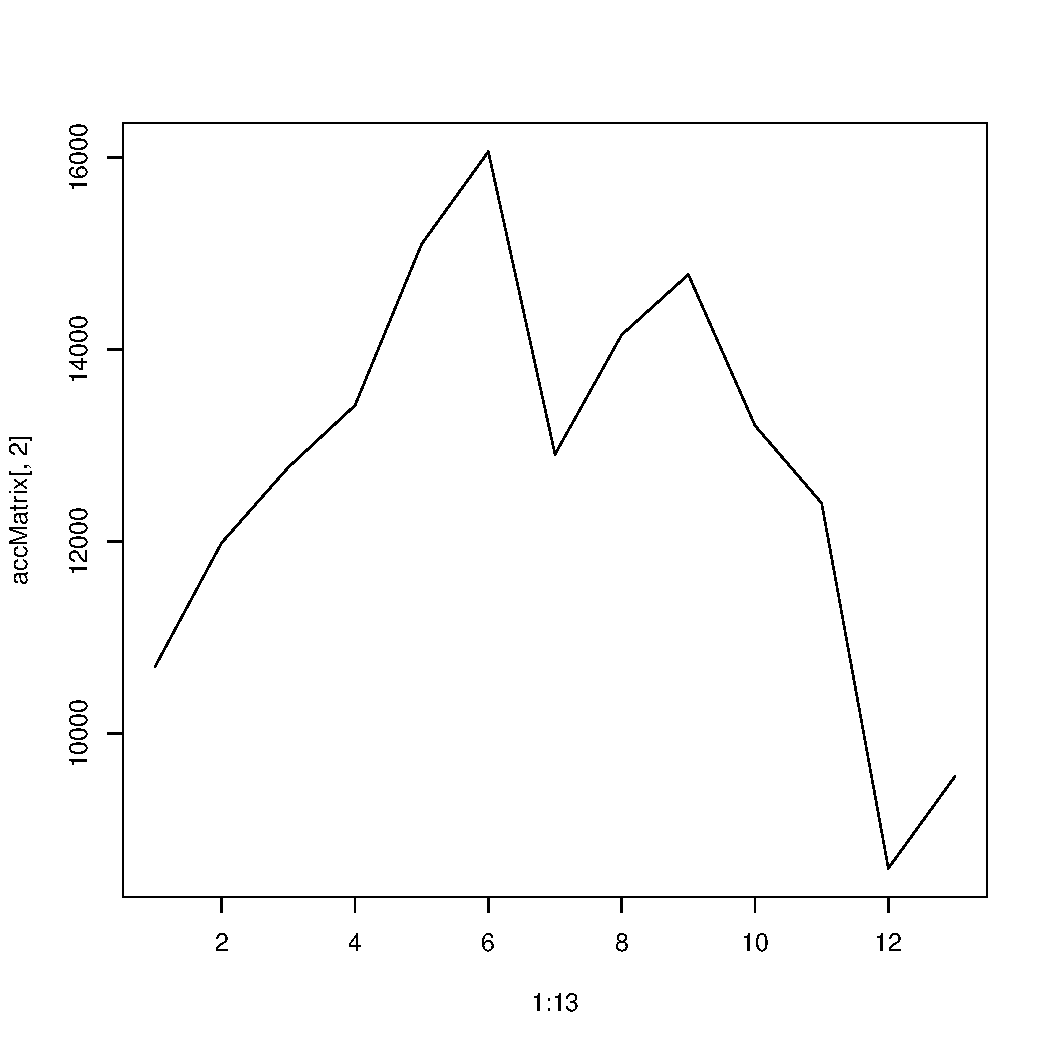
\includegraphics[width=0.33\textwidth]{../imagenes/segundoPeriodo.pdf}}
  \subfloat[Tercer periodo]{
   \label{f:periodo3}
    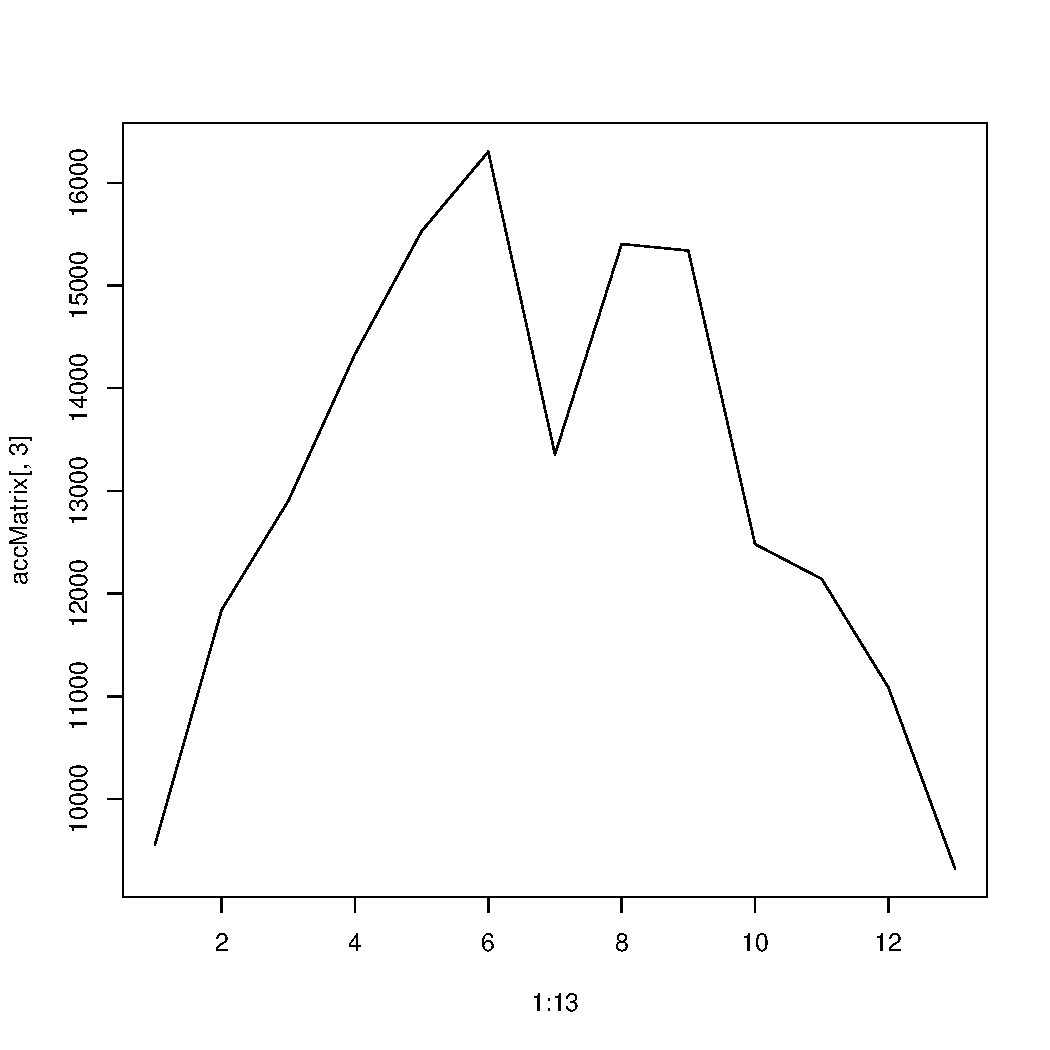
\includegraphics[width=0.33\textwidth]{../imagenes/tercerPeriodo.pdf}}
 \caption{Primeros periodos de la serie de accidentes en Italia}
 \label{f:periodos}
\end{figure}
\end{frame}

\note{Aquí se muestran los 3 primeros intervalos de 13 puntos de la serie original. Esto se ha hecho implementando una pequeña función en \texttt{R} que devuelve directamente la matriz con las series como columnas. Lo siguiente es poner todas estas series en una matriz, por columnas, y utilizar el algoritmo \texttt{gdpc} de forma que sólo se obtenga una componente principal dinámica. Esto no es difícil puesto que las series deben parecerse mucho entre sí al ser la serie original periódica y aumentando el número de lags a utilizar o disminuyendo un poco la varianza a explicar, se consigue. En este caso, la única componente principal dinámica es la que aparece en la siguiente diapositiva.}

\begin{frame}{Aplicación a detección de patrones en series temporales periódicas}
\begin{figure}[]
 \centering
 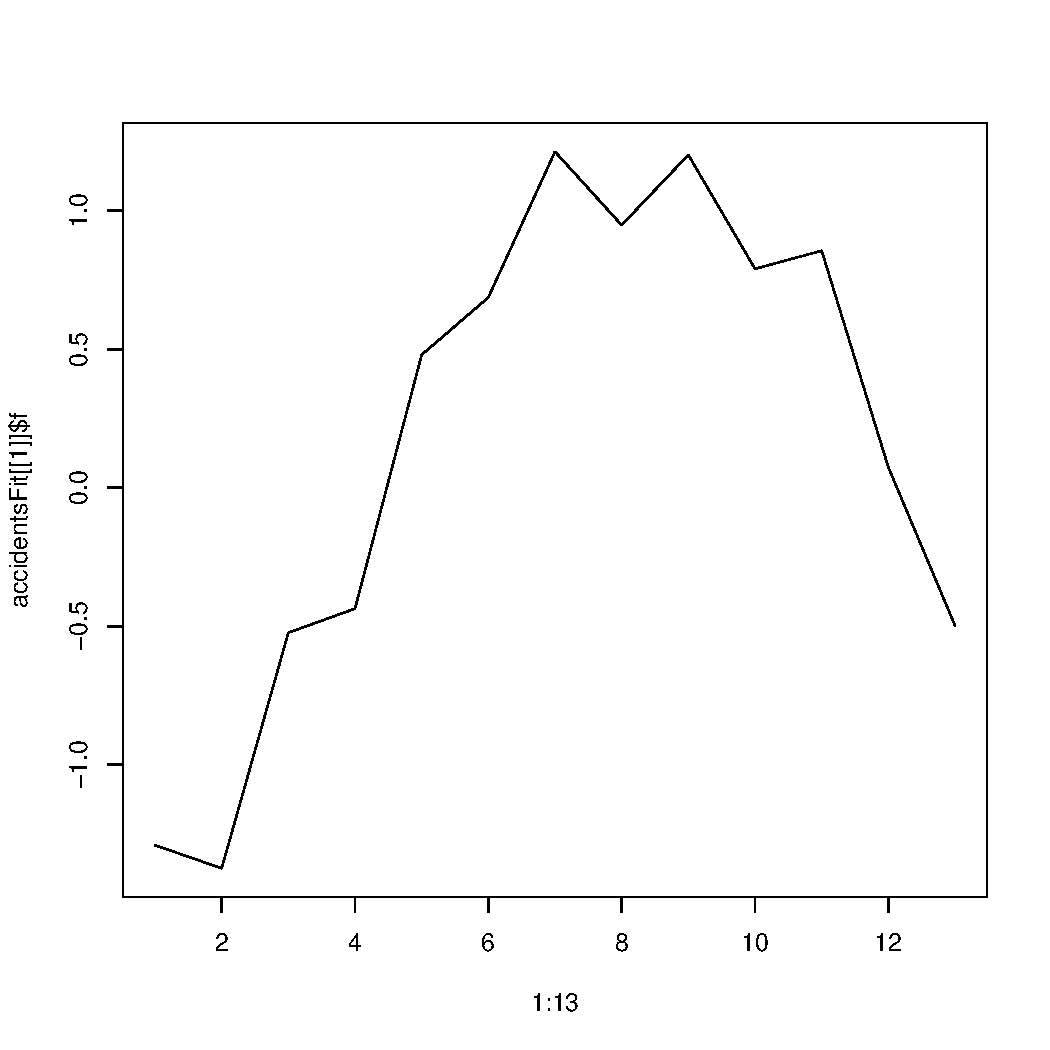
\includegraphics[width=0.5\textwidth]{../imagenes/accidentsComp.pdf}
 \caption{Componente principal dinámica para la serie de accidentes}
 \label{f:accidentsComp}
\end{figure}
\end{frame}

\begin{frame}{Aplicación a predicción de nuevos valores de un conjunto de series temporales}
\begin{equation}
\widehat{z}_{j,t} = \sum_{i=0}^{k} \beta_{j,i+1}f_{t+i} + \alpha_j
\end{equation}

Con series de 5 valores y reconstruyendo con $k=4$ leads, si queremos obtener el sexto valor de la primera serie sólo nos hace falta predecir el primer siguiente valor de $\mathbf{f}$, $\widehat{f}_{10}$, y la reconstrucción sería:
\begin{equation}
\widehat{z}_{1,6} = \beta_{1,1}f_6 + \beta_{1,2}f_7 + \beta_{1,3}f_8 + \beta_{1,4}f_9 + \beta_{1,5}\widehat{f}_{10} + \alpha_1
\end{equation}

\end{frame}

\note{Lo que queremos hacer es predecir nuevos valores de un conjunto de series temporales (que puede ser tan grande como se quiera), que es una de las prácticas más comunes en el análisis de series temporales, a través de la predicción de nuevos valores de las componentes principales, que normalmente es un conjunto mucho más pequeño de series, lo que facilita la predicción. La reconstrucción con $k$ leads, como hemos visto antes, es la que aparece en la diapositiva. Como vemos, el único parámetro que depende de $t$, que es el valor de la serie que se está reconstruyendo, es $f$. Esto significa que si obtenemos más valores de $f$, podemos reconstruir más valores de $z$, las series reconstruidas.}

\note{Esto tiene el inconveniente de que a más valores intentemos predecir de $\mathbf{f}$ peor serán los valores obtenidos al hacer la reconstrucción porque los coeficientes, tanto $\beta$ como $\alpha$ se han generado con los valores conocidos de las series originales y no tienen por qué funcionar también para los valores predichos de $\mathbf{f}$. Sin embargo, este es un problema presente siempre que se trata la predicción de series temporales: a mayor horizonte de predicción, menos fiables son los resultados.}

\begin{frame}{Aplicación a predicción de nuevos valores de un conjunto de series temporales}
\begin{figure}[]
 \centering
  \subfloat[Serie original]{
   \label{f:franciaO}
    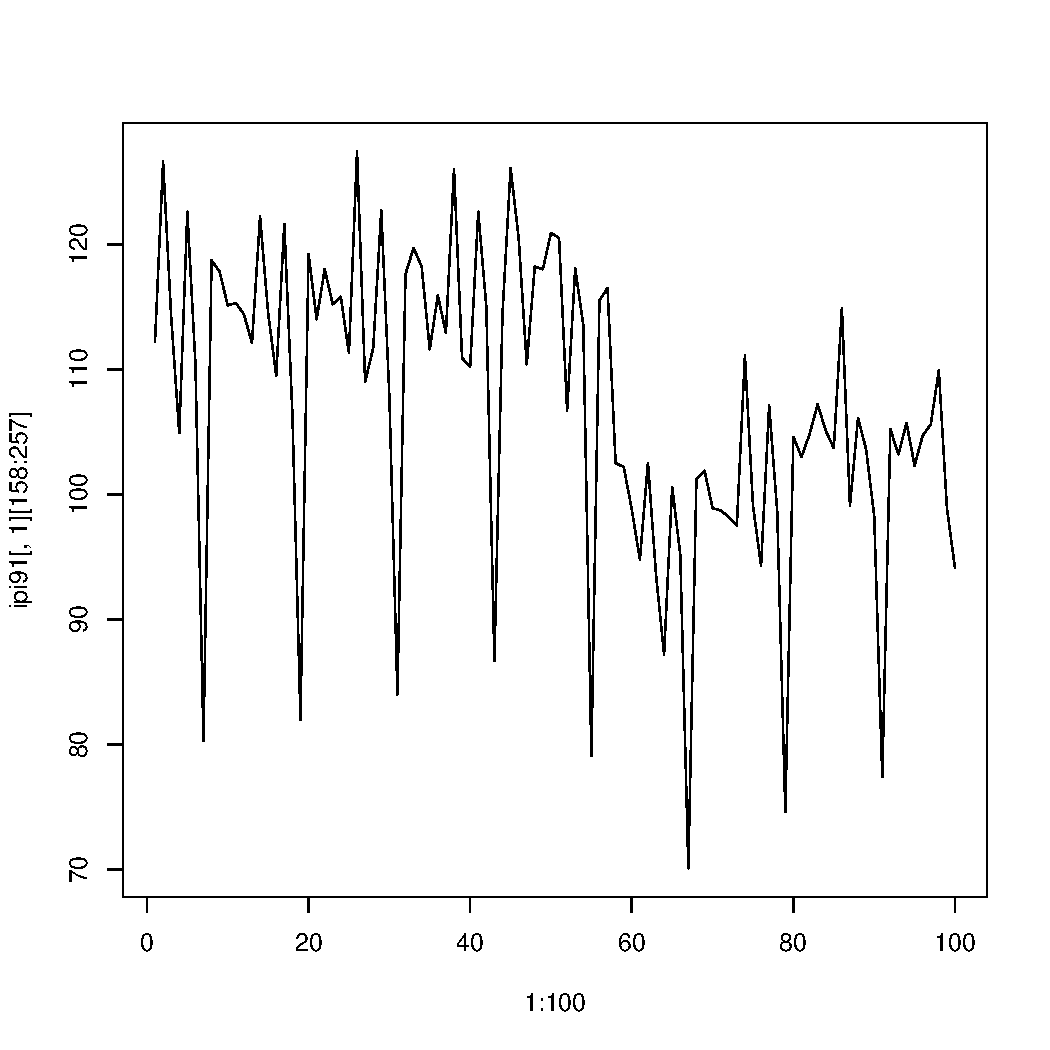
\includegraphics[width=0.33\textwidth]{../imagenes/ipi1original.pdf}}
  \subfloat[Reconstrucción con AR(2)]{
   \label{f:franciaAR}
    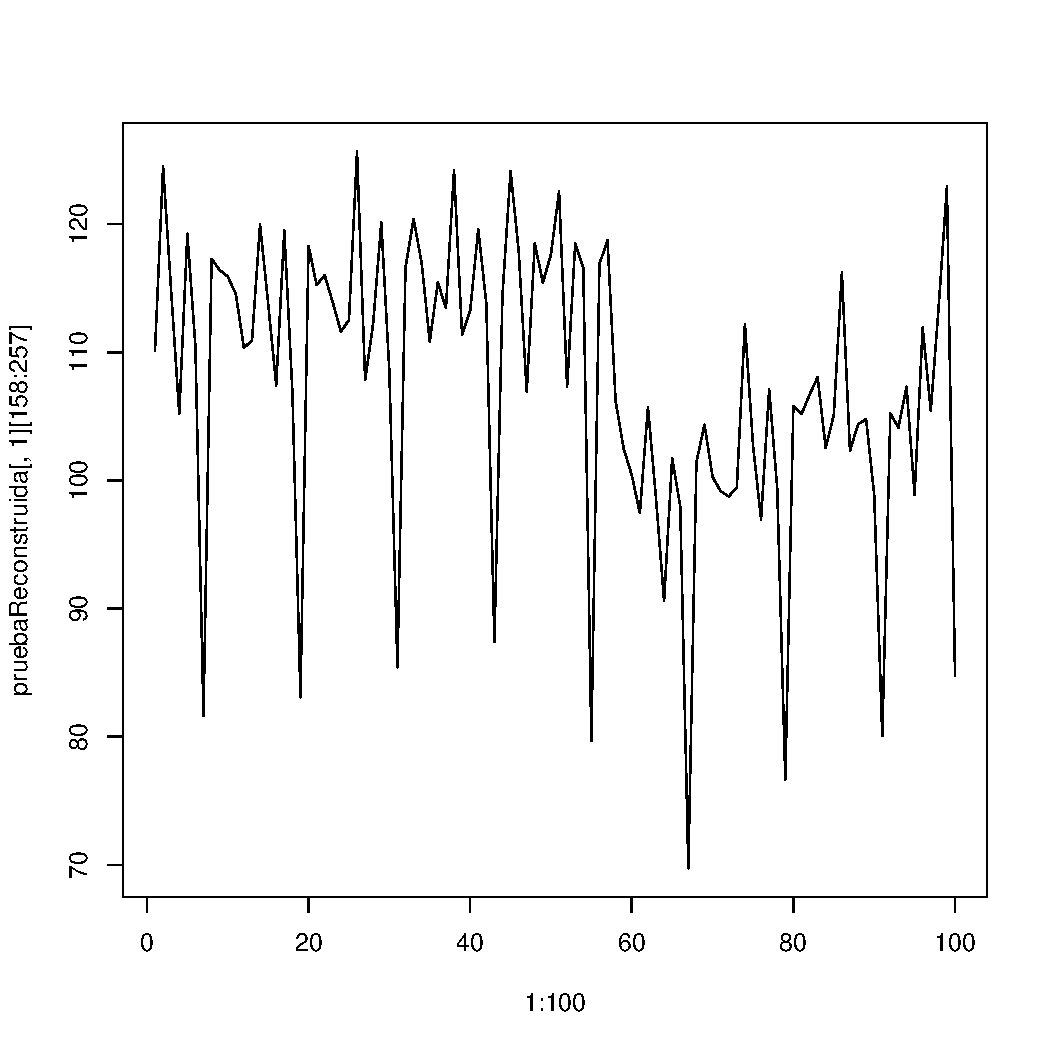
\includegraphics[width=0.33\textwidth]{../imagenes/ipi1ar.pdf}}
  \subfloat[Reconstrucción con ARMA(2,2)]{
  \centering
   \label{f:franciaARMA}
    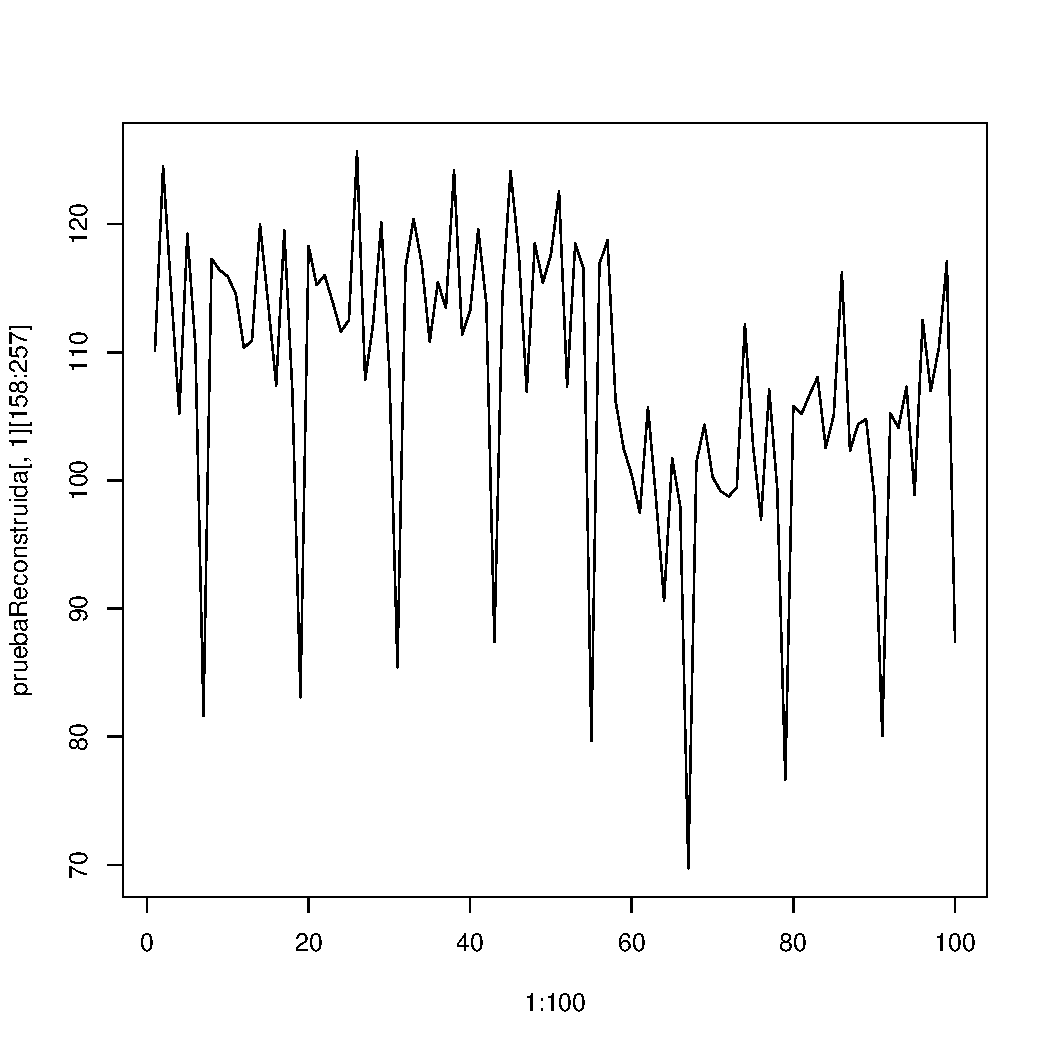
\includegraphics[width=0.33\textwidth]{../imagenes/ipi1arma.pdf}}
 \caption{IPI en Francia}
 \label{f:francia}
\end{figure}
\end{frame}

\note{Estos experimentos se han hecho con un conjunto de datos perteneciente al paquete \texttt{gdpc} con el índice de producción industrial de cuatro países. Se han cogido 12 valores menos de cada serie al sacar las componentes principales dinámicas para tener valores con los que comparar al hacer la reconstrucción de las predicciones. Se ha obtenido una componente principal y se ha modelado con un modelo AR(2) y con modelo ARMA(2,2), obteniendo con cada uno de ellos los 5 siguientes valores, y se ha hecho la reconstrucción de los valores originales con los valores devueltos por ambos modelos. En estas figuras vemos los últimos 100 valores de cada serie, incluyendo los 5 valores predichos. Como vemos no difieren mucho de los valores originales, obteniéndose unos valores predichos buenos, aunque según aumenta el horizonte de predicción se van alejando más de los originales.}

\begin{frame}{Aplicación a predicción de nuevos valores de un conjunto de series temporales}
\begin{figure}[]
 \centering
  \subfloat[Serie original]{
   \label{f:alemaniaO}
    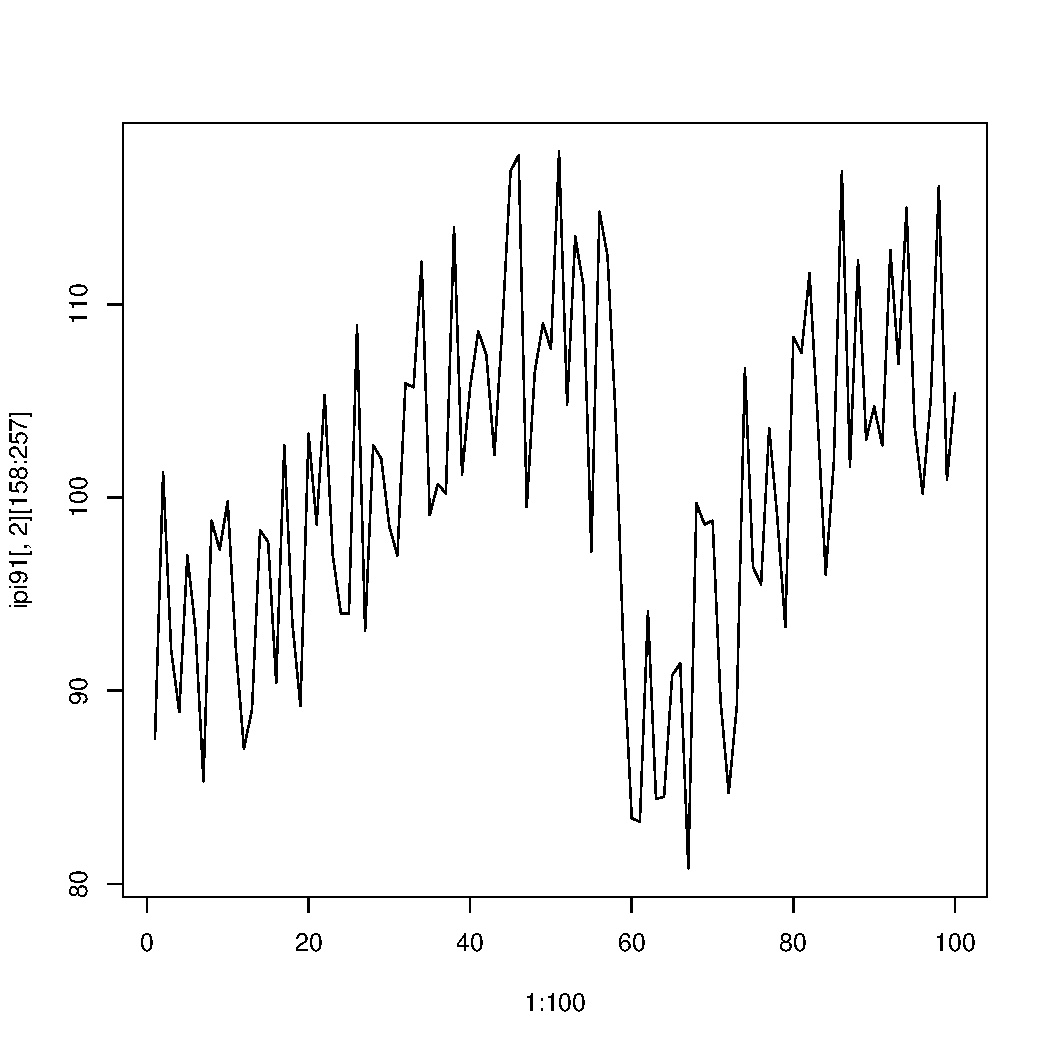
\includegraphics[width=0.33\textwidth]{../imagenes/ipi2original.pdf}}
  \subfloat[Reconstrucción con AR(2)]{
   \label{f:alemaniaAR}
    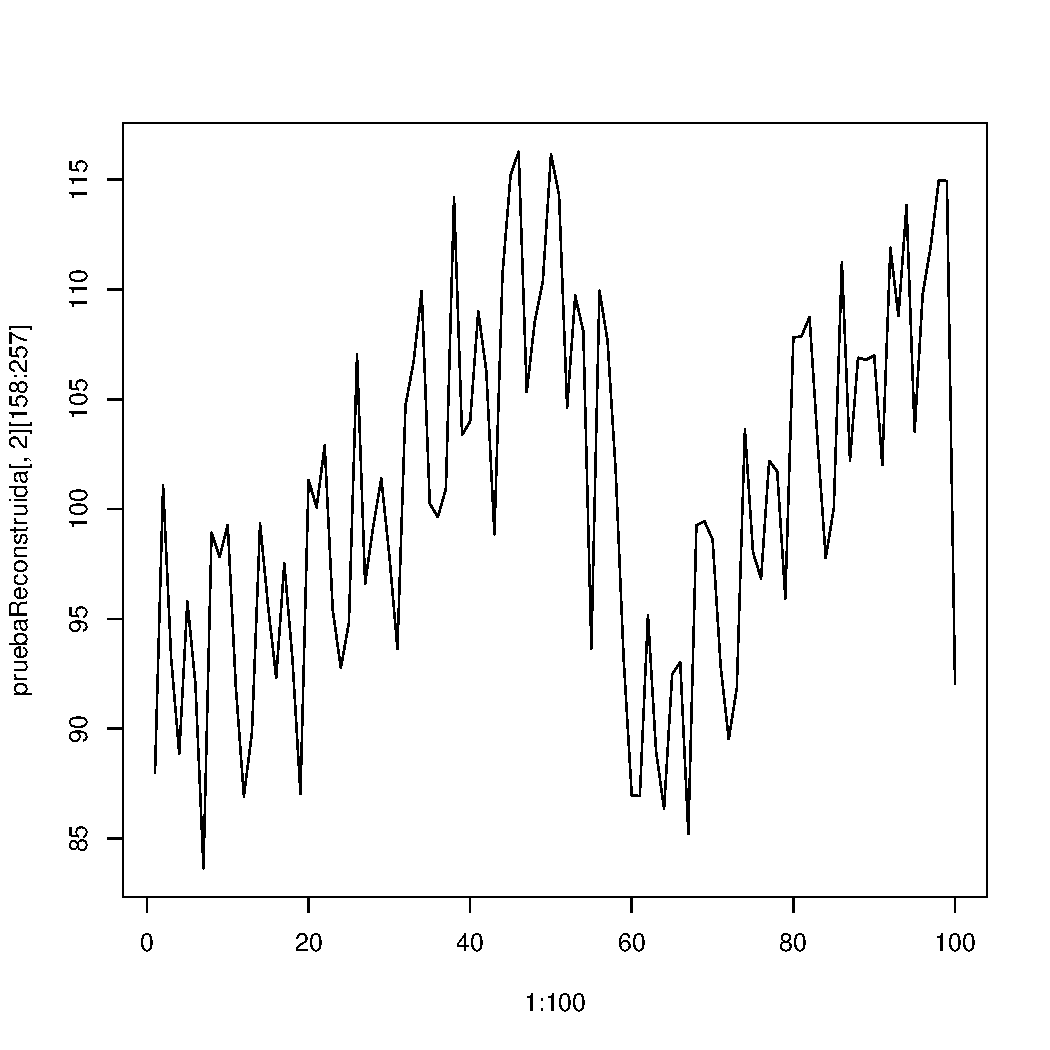
\includegraphics[width=0.33\textwidth]{../imagenes/ipi2ar.pdf}}
  \subfloat[Reconstrucción con ARMA(2,2)]{
  \centering
   \label{f:alemaniaARMA}
    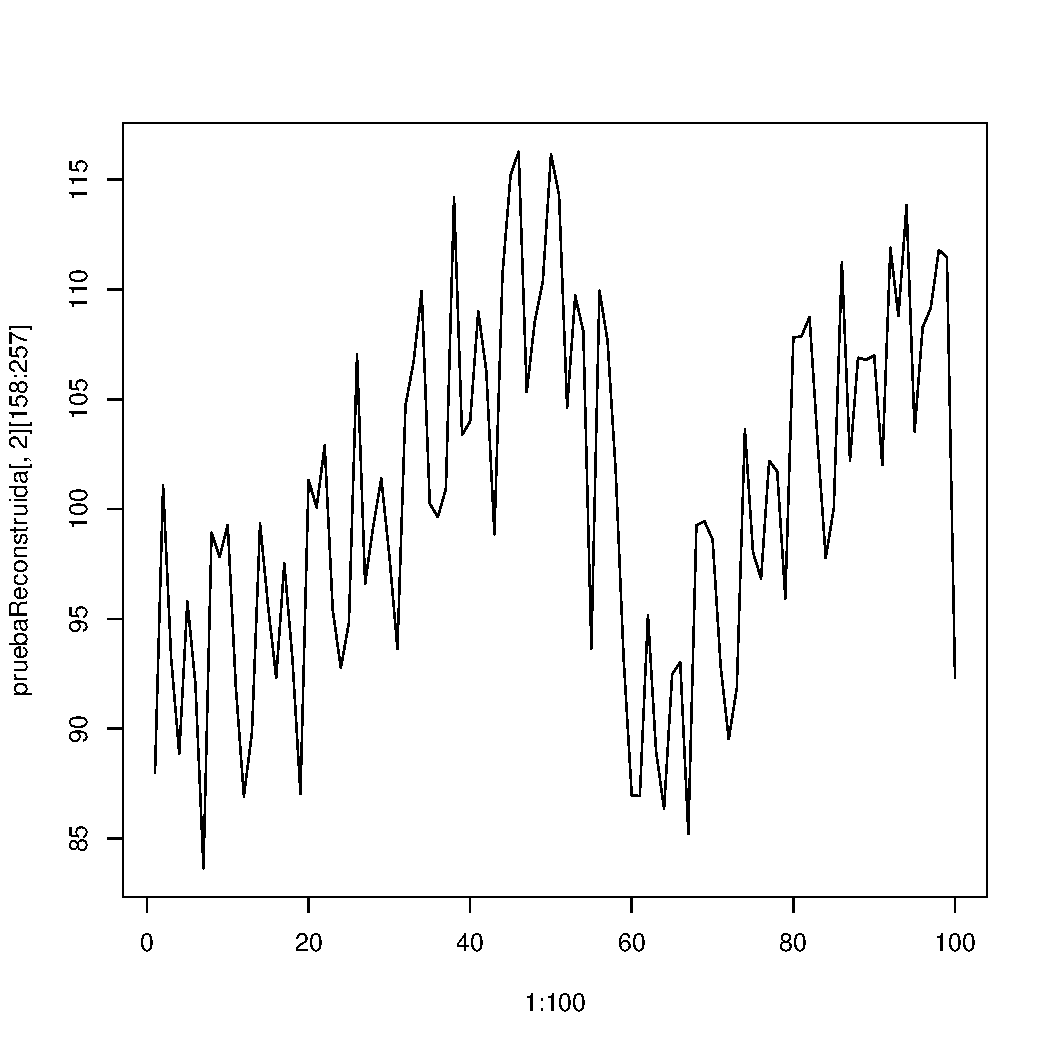
\includegraphics[width=0.33\textwidth]{../imagenes/ipi2arma.pdf}}
 \caption{IPI en Alemania}
 \label{f:alemania}
\end{figure}
\end{frame}

\note{En este caso los valores predichos son peores que en el caso anterior. Hay que tener en cuenta que se han obtenido los valores predichos con dos modelos lineales simples y que convendría hacerlo con otros modelos, que dieran mejores predicciones de la componente principal y por tanto mejores resultados al reconstruir las series y obtener valores predichos de las series originales.}

\section{Conclusiones y vías futuras}

\begin{frame}
\begin{enumerate}
\item Se ha estudiado si esta nueva técnica se puede utilizar en compresión de imágenes y se han realizado experimentos que han dado mejores resultados que los que se esperaban inicialmente. Aun así, el tiempo en comprimir una imagen es alto para esta aplicación.
\item Se pueden, a partir de ahora, seguir buscando aplicaciones de dicho método.
\item Conviene también seguir experimentando para mejorar las dos últimas aplicaciones. Especialmente utilizar otros métodos de predicción más avanzados a la hora de predecir valores de las componentes principales dinámicas para mejorar la predicción del conjunto de series originales.
\end{enumerate}
\end{frame}

\end{document}
